\documentclass[aspectratio=169,11pt]{beamer}

\usepackage[utf8]{inputenc}
\usepackage[T1]{fontenc}
\usepackage[spanish]{babel}
\usepackage{amsmath,amssymb}
\usepackage{graphicx}
\usepackage{tikz}
\usepackage{array}
\usepackage{booktabs}

\usetheme{default}
\setbeamertemplate{navigation symbols}{}
\setbeamertemplate{footline}[frame number]

\definecolor{preuvbg}{HTML}{FBF7EF}
\definecolor{preuvdark}{HTML}{2C2C2C}
\definecolor{preuvgold}{HTML}{E0A456}
\definecolor{preuvmuted}{HTML}{6F6A61}
\definecolor{preuvred}{HTML}{F23B35}
\definecolor{preuvblue}{HTML}{2BB5C6}

\setbeamercolor{background canvas}{bg=preuvbg}
\setbeamercolor{normal text}{fg=preuvdark}
\setbeamercolor{frametitle}{fg=preuvdark}
\setbeamercolor{structure}{fg=preuvgold}
\setbeamercolor{block title}{bg=preuvgold!18,fg=preuvdark}
\setbeamercolor{block body}{bg=white,fg=preuvdark}

\setbeamerfont{frametitle}{size=\Large,series=\bfseries}
\setbeamerfont{title}{size=\Huge,series=\bfseries}
\setbeamerfont{subtitle}{size=\large}

\newcommand{\pregunta}[1]{%
  \begin{center}
  \setlength{\fboxsep}{10pt}
  \colorbox{preuvgold!12}{\(\displaystyle #1\)}
  \end{center}
}

\newcommand{\caja}[1]{%
  \begin{center}
  \setlength{\fboxsep}{9pt}
  \colorbox{white}{\(\displaystyle \boxed{#1}\)}
  \end{center}
}

\newcommand{\smallnote}[1]{%
  \vspace{0.4em}
  {\small\color{preuvmuted}#1}
}

\title{Movimiento Rectilíneo Uniforme}
\subtitle{¿Cómo transformamos el movimiento real en una descripción matemática?}
\author{Profesor Joaquín Saldaño}
\institute{Preuniversitario Solidario PREUV}
\date{}

\begin{document}

\begin{frame}
  \titlepage
  % Guion oral: abrir con la pregunta central. La clase no parte con fórmula,
  % parte con el problema de representar matemáticamente un movimiento real.
\end{frame}

\begin{frame}{¿Cómo describimos el movimiento?}
  \pregunta{\text{¿Qué significa decir que algo se mueve?}}
  \vspace{0.5em}
  Decir ``la pelota se mueve'' es incompleto.
  \begin{itemize}
    \item ¿Se mueve respecto de qué?
    \item ¿Dónde estaba antes?
    \item ¿Dónde está ahora?
    \item ¿Cuánto tiempo pasó?
  \end{itemize}
  \caja{\text{Movimiento}=\text{cambio de posición respecto de una referencia}}
  % Guion oral: insistir en que movimiento es comparación entre posiciones en distintos instantes.
\end{frame}

\begin{frame}{La posición no existe sola}
  \caja{\text{Toda posición es relativa a una referencia}}
  \vspace{0.6em}
  Una persona sentada dentro de un bus:
  \begin{itemize}
    \item respecto del asiento, está en reposo;
    \item respecto de la calle, está en movimiento.
  \end{itemize}
  \vspace{0.5em}
  Las dos afirmaciones pueden ser correctas.
  \begin{center}
  \begin{tikzpicture}[scale=0.85]
    \draw[very thick] (0,0) rectangle (5.8,1.2);
    \draw[fill=preuvdark] (1,-0.15) circle (0.25);
    \draw[fill=preuvdark] (4.8,-0.15) circle (0.25);
    \draw[fill=preuvgold] (2.9,0.65) circle (0.18);
    \draw[->,very thick,preuvgold] (-0.2,1.8)--(6.2,1.8);
    \node at (3,-0.8) {reposo respecto del asiento};
  \end{tikzpicture}
  \end{center}
  % Guion oral: no existe contradicción, existen sistemas de referencia distintos.
\end{frame}

\begin{frame}{El sistema de referencia}
  Un sistema de referencia necesita:
  \caja{\text{origen}+\text{dirección}+\text{sentido}+\text{unidad}+\text{reloj}}
  \begin{align*}
    x=0,\qquad
    \text{derecha}&\longrightarrow x>0,\\
    \text{izquierda}&\longrightarrow x<0.
  \end{align*}
  \begin{center}
  \begin{tikzpicture}[scale=0.9]
    \draw[->,very thick] (-4,0)--(4.2,0);
    \foreach \x in {-3,-2,-1,0,1,2,3} {
      \draw (\x,0.1)--(\x,-0.1);
      \node[below] at (\x,-0.1) {\x};
    }
    \node[above,preuvgold] at (0,0.2) {origen};
  \end{tikzpicture}
  \end{center}
  % Guion oral: la naturaleza no trae flechas positivas dibujadas; el sentido es una elección.
\end{frame}

\begin{frame}{Convertir el espacio en números}
  \begin{align*}
    \text{lugar físico} &\longrightarrow \text{número}\\
    P &\longrightarrow x(P)
  \end{align*}
  \vspace{0.5em}
  Una coordenada permite reemplazar frases vagas por mediciones:
  \[
    \text{``un poco más allá del árbol''}
    \quad\longrightarrow\quad
    x=12\,\mathrm{m}.
  \]
  \caja{\text{Una coordenada es una etiqueta numérica para una posición}}
  % Guion oral: el número no es la realidad; es la representación dentro del sistema elegido.
\end{frame}

\begin{frame}{¿Por qué usamos una recta?}
  \caja{\text{movimiento en una sola dimensión}}
  \vspace{0.5em}
  En MRU suponemos que una coordenada basta:
  \[
    x.
  \]
  \[
    \text{realidad compleja}
    \longrightarrow
    \text{modelo simplificado}.
  \]
  \begin{center}
  \begin{tikzpicture}
    \draw[very thick,gray!45,line width=8pt] (-4,0).. controls (-1,1) and (1,1)..(4,0);
    \draw[very thick,->] (-3.7,0)--(3.9,0);
    \draw[fill=preuvgold] (1.6,0) circle (0.18);
    \node[below] at (0,-0.25) {modelo 1D};
  \end{tikzpicture}
  \end{center}
  % Guion oral: modelo no significa mentira; significa conservar lo relevante para la pregunta.
\end{frame}

\begin{frame}{Geometría euclidiana}
  En nuestro modelo suponemos:
  \caja{\text{un espacio plano}}
  \begin{itemize}
    \item por dos puntos pasa una única recta;
    \item el camino recto es el camino más corto;
    \item las distancias se calculan con Pitágoras.
  \end{itemize}
  \[
    d=\sqrt{(x_2-x_1)^2+(y_2-y_1)^2},
    \qquad
    d=|x_2-x_1| \quad \text{en una dimensión}.
  \]
  % Guion oral: dedicar poco tiempo. Esto es marco conceptual, no el tema principal.
\end{frame}

\begin{frame}{¿La Tierra es plana?}
  \caja{\text{No globalmente, pero puede aproximarse como plana localmente}}
  \vspace{0.4em}
  \[
    \text{pequeña región}
    \Rightarrow
    \text{aproximación plana}.
  \]
  \begin{center}
  \begin{tikzpicture}[scale=0.8]
    \shade[ball color=preuvblue!70] (0,0) circle (1.4);
    \draw[preuvgold,very thick] (-0.45,0.45).. controls (0,0.75) and (0.55,0.68)..(0.85,0.42);
    \draw[->,thick] (1.25,0.65)--(2.7,0.95);
    \draw[fill=white,thick] (3,0.25) rectangle (5.5,1.45);
    \draw[preuvgold,very thick] (3.35,0.85)--(5.15,0.85);
    \node at (4.25,-0.15) {la curva se ve casi plana};
  \end{tikzpicture}
  \end{center}
  % Guion oral: no estamos afirmando que la Tierra sea plana; usamos una aproximación local.
\end{frame}

\begin{frame}{Cuando el plano deja de funcionar}
  \caja{\text{En espacios curvos cambian las reglas geométricas}}
  \vspace{0.3em}
  En una esfera:
  \begin{itemize}
    \item el camino más corto es un arco de círculo máximo;
    \item los triángulos pueden tener más de \(180^\circ\);
    \item las coordenadas cartesianas dejan de ser las más naturales.
  \end{itemize}
  \begin{center}
    \IfFileExists{assets/spherical-triangle.png}
      {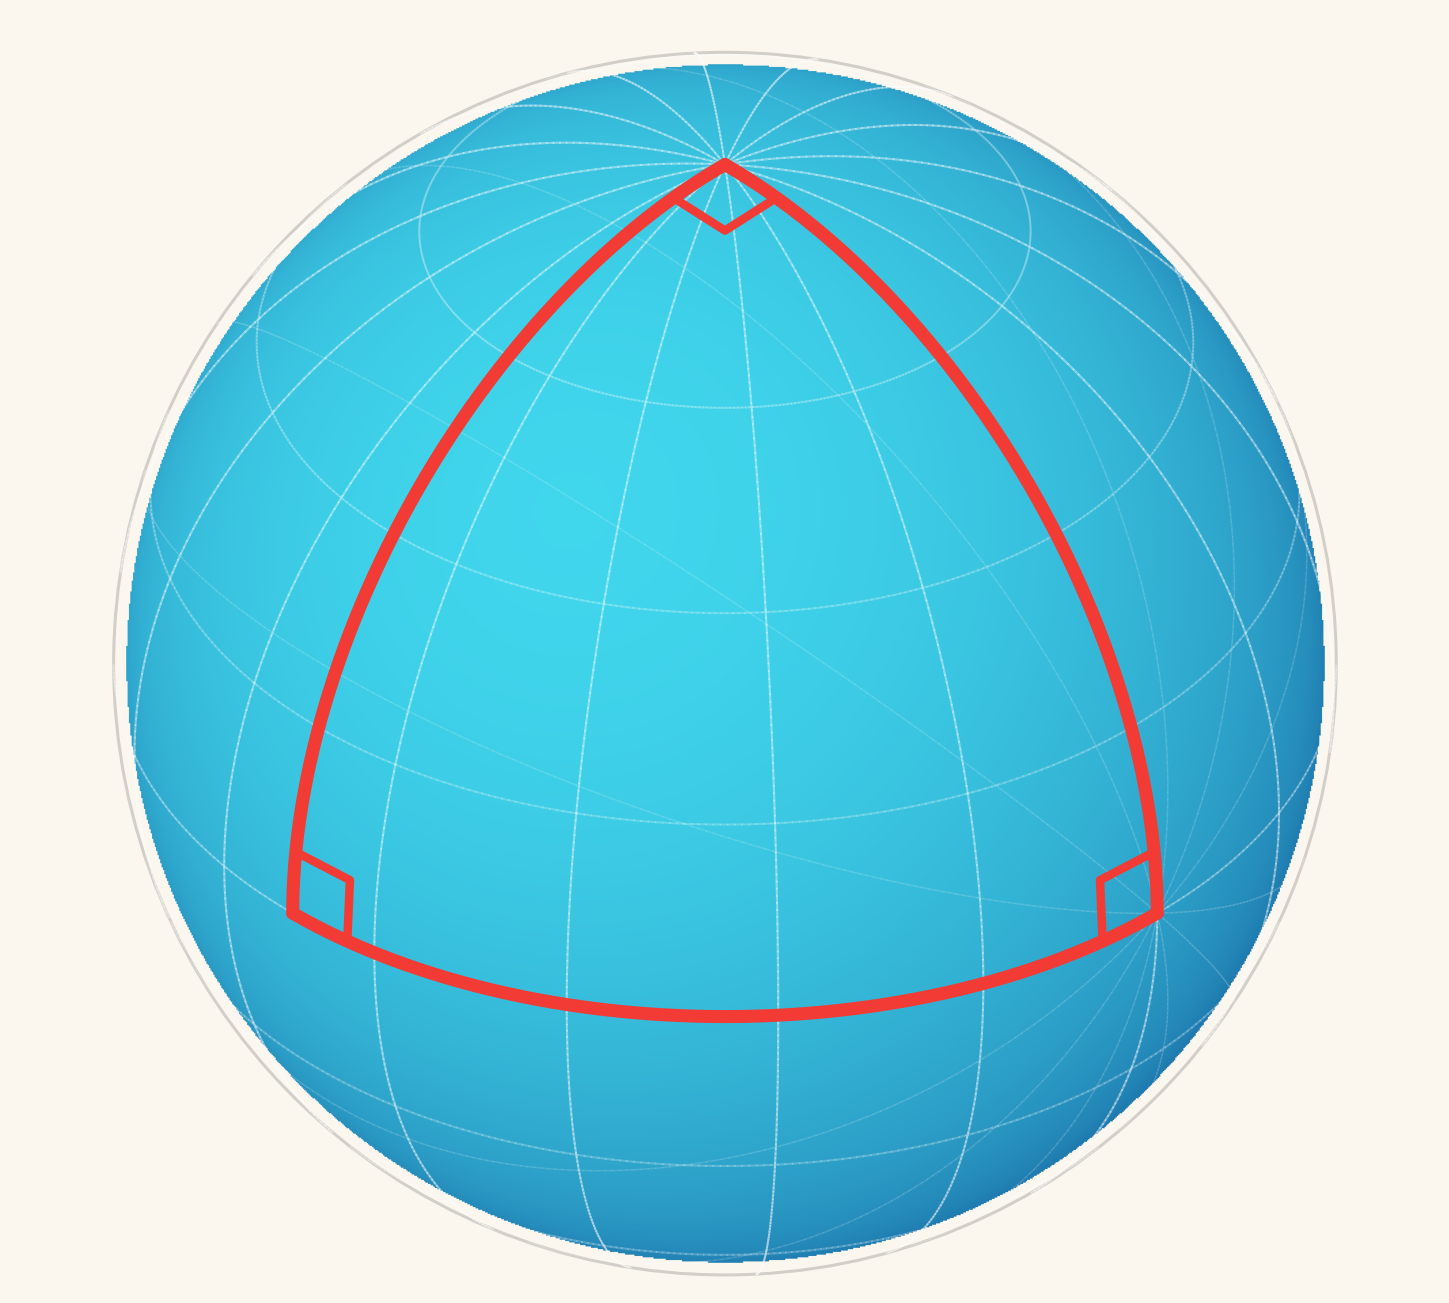
\includegraphics[height=3.0cm]{assets/spherical-triangle.png}}
      {\IfFileExists{spherical-triangle.png}
        {
\includegraphics[height=3.0cm]{spherical-triangle.png}}
        {\fbox{\parbox{6.5cm}{Subir a Overleaf el archivo \texttt{spherical-triangle.png}}}}}
  \end{center}
  \caja{\text{El MRU escolar supone un espacio localmente plano}}
  % Guion oral: usar esta diapositiva como ejemplo visual breve, no como clase de geometría diferencial.
\end{frame}

\begin{frame}{Espacio físico y espacio-tiempo}
  Para esta clase suponemos:
  \caja{\text{espacio euclidiano}+\text{tiempo universal}}
  \vspace{0.5em}
  Esta aproximación funciona bien para:
  \begin{itemize}
    \item autos, personas, pelotas y trenes;
    \item velocidades pequeñas comparadas con \(c\);
    \item regiones pequeñas;
    \item campos gravitatorios no extremos.
  \end{itemize}
  % Guion oral: toda teoría tiene dominio de validez. MRU no es falso; tiene contexto.
\end{frame}

\begin{frame}{¿Qué es un gráfico?}
  \caja{\text{Un gráfico representa la relación entre variables}}
  \vspace{0.5em}
  En un gráfico posición-tiempo:
  \begin{itemize}
    \item el eje horizontal representa el tiempo;
    \item el eje vertical representa la posición.
  \end{itemize}
  \[
    (3\,\mathrm{s},12\,\mathrm{m})
  \]
  significa: a los \(3\,\mathrm{s}\), la posición era \(12\,\mathrm{m}\).
  \caja{\text{Un gráfico es un espacio de información}}
  % Guion oral: recalcar que el gráfico no es necesariamente el dibujo del camino físico.
\end{frame}

\begin{frame}{¿Por qué el tiempo va en el eje horizontal?}
  \[
    t\longrightarrow \text{variable independiente}
  \]
  \[
    x(t)\longrightarrow \text{variable dependiente}
  \]
  \vspace{0.4em}
  La notación \(x(t)\) se lee:
  \[
    \text{posición en función del tiempo}.
  \]
  No significa \(x\) multiplicado por \(t\).
  \[
    x(0),\qquad x(1),\qquad x(2).
  \]
  % Guion oral: el tiempo es la entrada; la posición es el resultado.
\end{frame}

\begin{frame}{¿Existen otros tipos de gráficos?}
  \caja{\text{Sí. Elegimos la representación según el problema}}
  \begin{itemize}
    \item coordenadas cartesianas \((x,y)\);
    \item coordenadas polares \((r,\theta)\);
    \item coordenadas cilíndricas y esféricas;
    \item gráficos posición-tiempo y velocidad-tiempo.
  \end{itemize}
  \[
    \text{movimiento recto}\Rightarrow x,
    \qquad
    \text{movimiento circular}\Rightarrow r,\theta.
  \]
  % Guion oral: las coordenadas cambian la descripción, no el fenómeno físico.
\end{frame}

\begin{frame}{Movimiento como función}
  \caja{x=x(t)}
  \[
  \begin{array}{c|ccccc}
  t\,(\mathrm{s}) & 0 & 1 & 2 & 3 & 4\\
  \hline
  x\,(\mathrm{m}) & 2 & 5 & 8 & 11 & 14
  \end{array}
  \]
  \[
    t\longmapsto x(t)
  \]
  Entrada: tiempo. \qquad Salida: posición.
  % Guion oral: función significa una salida para cada entrada permitida.
\end{frame}

\begin{frame}{¿Qué está cambiando?}
  \[
    \Delta x=x_f-x_i,
    \qquad
    \Delta t=t_f-t_i.
  \]
  Si
  \[
    x_i=2\,\mathrm{m},\qquad x_f=8\,\mathrm{m},
  \]
  entonces
  \[
    \Delta x=8-2=6\,\mathrm{m}.
  \]
  Si
  \[
    t_i=0\,\mathrm{s},\qquad t_f=2\,\mathrm{s},
  \]
  entonces
  \[
    \Delta t=2\,\mathrm{s}.
  \]
  % Guion oral: Delta significa diferencia, no una variable nueva misteriosa.
\end{frame}

\begin{frame}{Razón de cambio}
  \caja{v=\dfrac{\Delta x}{\Delta t}}
  En el ejemplo:
  \[
    v=\frac{6\,\mathrm{m}}{2\,\mathrm{s}}
    =3\,\frac{\mathrm{m}}{\mathrm{s}}.
  \]
  Esto significa:
  \[
    \text{por cada segundo, la posición aumenta tres metros}.
  \]
  \[
    v>0,\qquad v<0,\qquad v=0.
  \]
  % Guion oral: velocidad no es solo rapidez; también informa sentido.
\end{frame}

\begin{frame}{¿Qué hace uniforme al MRU?}
  \caja{\dfrac{\Delta x}{\Delta t}=\text{constante}}
  \[
  \begin{array}{c|ccccc}
  t\,(\mathrm{s}) & 0 & 1 & 2 & 3 & 4\\
  \hline
  x\,(\mathrm{m}) & 2 & 5 & 8 & 11 & 14
  \end{array}
  \]
  \[
    5-2=3,\qquad 8-5=3,\qquad 11-8=3,\qquad 14-11=3.
  \]
  La velocidad es constante.
  % Guion oral: uniforme no significa quieto; significa razón de cambio constante.
\end{frame}

\begin{frame}{Construcción de la ecuación}
  Partimos de:
  \[
    v=\frac{x-x_0}{t-t_0}.
  \]
  Multiplicamos:
  \[
    v(t-t_0)=x-x_0.
  \]
  Sumamos \(x_0\):
  \[
    x=x_0+v(t-t_0).
  \]
  Si elegimos \(t_0=0\):
  \caja{x(t)=x_0+vt}
  % Guion oral: la fórmula aparece como consecuencia algebraica de velocidad constante.
\end{frame}

\begin{frame}{¿Qué significa cada término?}
  \caja{x(t)=x_0+vt}
  \begin{itemize}
    \item \(x(t)\): posición en el instante \(t\).
    \item \(x_0\): posición inicial.
    \item \(v\): cambio de posición por unidad de tiempo.
    \item \(vt\): cambio acumulado de posición.
  \end{itemize}
  \[
    \text{posición final}
    =
    \text{posición inicial}
    +
    \text{cambio de posición}.
  \]
  % Guion oral: conectar cada símbolo con una frase física.
\end{frame}

\begin{frame}{Es una función afín}
  Matemática:
  \[
    y=mx+b.
  \]
  Cinemática:
  \[
    x=vt+x_0.
  \]
  Correspondencia:
  \[
    y\leftrightarrow x,
    \qquad
    x\leftrightarrow t,
    \qquad
    m\leftrightarrow v,
    \qquad
    b\leftrightarrow x_0.
  \]
  % Guion oral: la función lineal aparece porque hay una razón de cambio constante.
\end{frame}

\begin{frame}{La pendiente es una razón de cambio}
  \caja{\text{pendiente}=\dfrac{\text{cambio vertical}}{\text{cambio horizontal}}}
  En posición-tiempo:
  \[
    \text{pendiente}
    =
    \frac{\Delta x}{\Delta t}
    =
    v.
  \]
  \begin{center}
  \begin{tikzpicture}[scale=0.85]
    \draw[->,thick] (0,0)--(6,0) node[right] {\(t\)};
    \draw[->,thick] (0,0)--(0,3.5) node[above] {\(x\)};
    \draw[preuvgold,very thick] (0.6,0.7)--(5.5,3.0);
    \draw[dashed] (2.2,1.45)--(4.5,1.45)--(4.5,2.52);
    \node at (3.3,1.15) {\(\Delta t\)};
    \node[right] at (4.5,2.0) {\(\Delta x\)};
  \end{tikzpicture}
  \end{center}
  % Guion oral: la pendiente tiene significado físico, no solo visual.
\end{frame}

\begin{frame}{Tres movimientos posibles}
  \[
    v>0\Rightarrow x(t)\text{ aumenta}
  \]
  \[
    v=0\Rightarrow x(t)\text{ permanece constante}
  \]
  \[
    v<0\Rightarrow x(t)\text{ disminuye}
  \]
  \[
    v=4\,\frac{\mathrm{m}}{\mathrm{s}},
    \qquad
    v=-4\,\frac{\mathrm{m}}{\mathrm{s}},
    \qquad
    |v|=4\,\frac{\mathrm{m}}{\mathrm{s}}.
  \]
  % Guion oral: velocidad negativa no significa menor rapidez; significa sentido negativo.
\end{frame}

\begin{frame}{El gráfico no es el camino}
  \caja{\text{trayectoria física}\neq \text{gráfico }x\text{-}t}
  \vspace{0.5em}
  Una recta inclinada en un gráfico posición-tiempo no significa que el objeto suba una pendiente física.
  \vspace{0.6em}
  Significa que:
  \[
    \text{la posición cambia uniformemente con el tiempo}.
  \]
  % Guion oral: separar el dibujo del camino real del espacio de información del gráfico.
\end{frame}

\begin{frame}{Ejemplo completo}
  \[
    x(t)=10-2t.
  \]
  Preguntas:
  \[
    x_0=?\qquad v=?\qquad x(3)=?
  \]
  Comparamos con \(x(t)=x_0+vt\):
  \[
    x_0=10\,\mathrm{m},
    \qquad
    v=-2\,\frac{\mathrm{m}}{\mathrm{s}}.
  \]
  \[
    x(3)=10-2(3)=4\,\mathrm{m}.
  \]
  % Guion oral: traducir el cálculo a historia física: parte en 10 m y se mueve al sentido negativo.
\end{frame}

\begin{frame}{Pregunta conceptual}
  Un móvil tiene:
  \[
    x(t)=5\,\mathrm{m}
  \]
  para todo \(t\).
  \vspace{0.5em}
  ¿Está en el origen?
  \vspace{0.5em}
  No necesariamente:
  \[
    x=5\,\mathrm{m}\quad\text{constante},
    \qquad
    v=0.
  \]
  \caja{\text{posición}\neq \text{velocidad}}
  % Guion oral: reposo no significa estar en x=0.
\end{frame}

\begin{frame}{El origen no tiene que ser el inicio}
  \caja{x_0\neq 0\text{ en general}}
  \[
    x=0
    \quad\text{es origen espacial.}
  \]
  \[
    t=0
    \quad\text{es inicio de la medición temporal.}
  \]
  \vspace{0.5em}
  Son elecciones distintas.
  \begin{center}
  \begin{tikzpicture}
    \draw[->,thick] (-4,0)--(4,0);
    \draw[fill=preuvdark] (-1.2,0) circle (0.07);
    \node[below] at (-1.2,-0.1) {\(x=0\)};
    \draw[fill=preuvgold] (2.0,0) circle (0.14);
    \node[above] at (2,0.2) {\(x_0=20\,\mathrm{m}\)};
  \end{tikzpicture}
  \end{center}
  % Guion oral: el móvil puede comenzar lejos del origen.
\end{frame}

\begin{frame}{Galileo, Newton y el MRU}
  \caja{\text{Galileo: describir el movimiento}}
  \caja{\text{Newton: formular leyes generales}}
  \vspace{0.4em}
  No es correcto presentar \(x=x_0+vt\) como una fórmula caída del cielo.
  \[
    \text{observaciones}
    \longrightarrow
    \text{conceptos}
    \longrightarrow
    \text{mediciones}
    \longrightarrow
    \text{relaciones matemáticas}.
  \]
  % Guion oral: Newton formaliza un marco general; Galileo ya había estudiado sistemáticamente el movimiento.
\end{frame}

\begin{frame}{¿Qué describe y qué no describe el MRU?}
  El MRU describe:
  \caja{\text{cómo cambia la posición}}
  No explica todavía:
  \caja{\text{por qué cambia el movimiento}}
  \vspace{0.5em}
  La cinemática describe el movimiento.
  \[
    \text{La dinámica estudiará sus causas.}
  \]
  % Guion oral: todavía no hablamos de fuerza, roce ni causas; solo descripción.
\end{frame}

\begin{frame}{Cierre}
  \[
    \boxed{
    \text{realidad}
    \rightarrow
    \text{referencia}
    \rightarrow
    \text{coordenadas}
    \rightarrow
    \text{mediciones}
    \rightarrow
    \text{función}}
  \]
  \[
    \boxed{
    v=\frac{\Delta x}{\Delta t}
    \quad\Longrightarrow\quad
    x(t)=x_0+vt}
  \]
  \vspace{0.5em}
  La fórmula final es la última etapa, no la primera.
  % Guion oral: cerrar volviendo a la pregunta inicial.
\end{frame}

\begin{frame}{Frase final}
  \caja{\text{Una fórmula física no es algo que hay que creer.}}
  \vspace{1em}
  \caja{\text{Es una relación que debemos aprender a construir e interpretar.}}
  % Guion oral: dejar esta frase como cierre lento, sin agregar más cálculo.
\end{frame}

\end{document}
